\begin{frame}{L'équation de Nagumo}{Contribution 1 | Comparaison ImEx - Splitting}
    \noindent\color{Primary}\rule{\linewidth}{0.6pt}\color{black}\\
        \textbf{L'équation de Nagumo 1D:\\}
        Il s'agit d'une équation de diffusion-réaction faisant apparaître des dynamiques de fronts :
            \begin{align}
                \partial_t{u} = \underbrace{D \partial_{xx}u}_{\text{diffusion}}
                        - \underbrace{ku(1-u^2)}_{\text{réaction non. lin.}}\quad k,D \in \mathbb{R^*_+}.
            \end{align}
    \pause
    \noindent\color{Primary}\rule{\linewidth}{0.6pt}\color{black}\\
        \textbf{Les solutions:\\}
            En domaine infini, cette équation admet des solutions sous forme d'ondes progressives :
        \begin{align}\label{eq:sol_nagumo}
            u(x-ct) = \frac{e^{\sqrt{\frac{k}{2D}} \bigl((x-x_0) - ct \bigr)}}
                        {1 + e^{-\sqrt{\frac{k}{2D}} \bigl((x-x_0) - ct \bigr)}},\quad c = \sqrt{\frac{kD}{2}}.
\end{align}
\centering
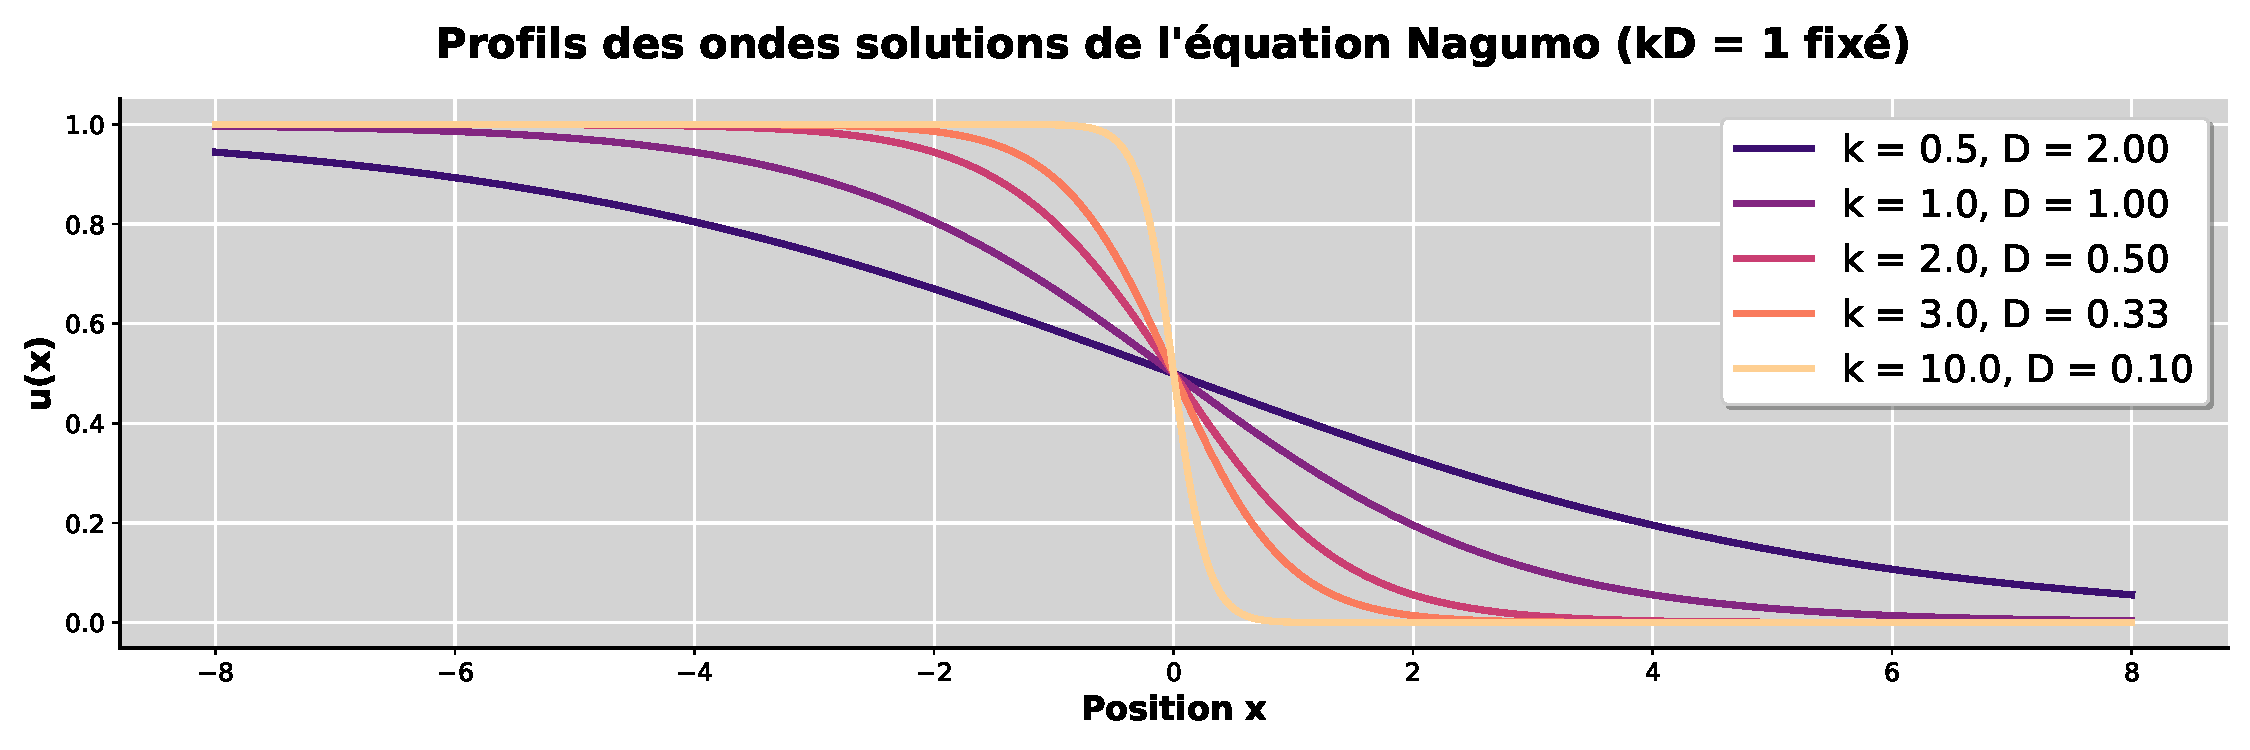
\includegraphics[height = .3 \textheight]{ medias/2_/1_/profils_nagumo.pdf }
\end{frame}